\subsection{Overview}
This chapter serves two roles.
It describes the implemented system, but it also justifies the empirical design used to answer the research questions.
The thesis is therefore structured as a comparative experimental study: the same warehouse environment, evaluation metrics, and scenario catalogue are reused while selected design variables are changed in order to study their effect on collaborative task performance.

This design is appropriate for the thesis because the research questions are comparative rather than purely descriptive.
RQ1 asks how model size affects performance, RQ2 asks how planning architecture affects performance, and RQ3 asks how prompt representation affects performance.
These questions require the report to make explicit what is fixed, what is varied, and how the experiments are structured across the objective families.

The thesis uses an empirical, experimental methodology:
\begin{enumerate}
    \item Implement an \gls{llm}-driven control loop for a simulated heterogeneous warehouse environment.
    \item Define the main comparison axes and evaluation metrics.
    \item Run controlled experiments (fixed environment ids and seeds) across multiple \gls{llm} models, planning architectures, and prompt variants.
    \item Analyze throughput, safety, and collaborative task outcomes as well as qualitative failure modes.
\end{enumerate}

\paragraph{What is fixed and what is varied.}
Across the main experiment families, the environment, action space, scenario catalogue, evaluation metrics, grounding/validation scheme, and local-inference setup are held as stable as practical.
The principal variables are model size, planning architecture, prompt representation, and objective family.
The report does not use an external heuristic baseline in the current comparison set, so the reported comparisons are made within the language-model-based control framework.

\paragraph{Interpretation and controls.}
The experiments are controlled in the sense that scenario ids, seeds, and runner configurations are recorded and reused within each family.
The surrounding validation layer filters infeasible outputs before execution, and the same comparison axes are used across the objective families.

\subsection{Environment: Battery-TA-RWARE}
Battery-TA-RWARE is a discrete-time, grid-based warehouse simulation derived from \gls{tarware}~\cite{krnjaic2024warehouse}.
At any time, a set of shelves is requested. Carrier \glspl{agv} must transport requested shelves to goal locations and then return them to storage.
Picker agents are required to meet \glspl{agv} at shelf locations for load and unload interactions, creating explicit heterogeneous coordination constraints.
Agents additionally have a battery state that decreases with movement and interactions; charging stations are available at fixed locations.

\begin{figure}[H]
    \centering
    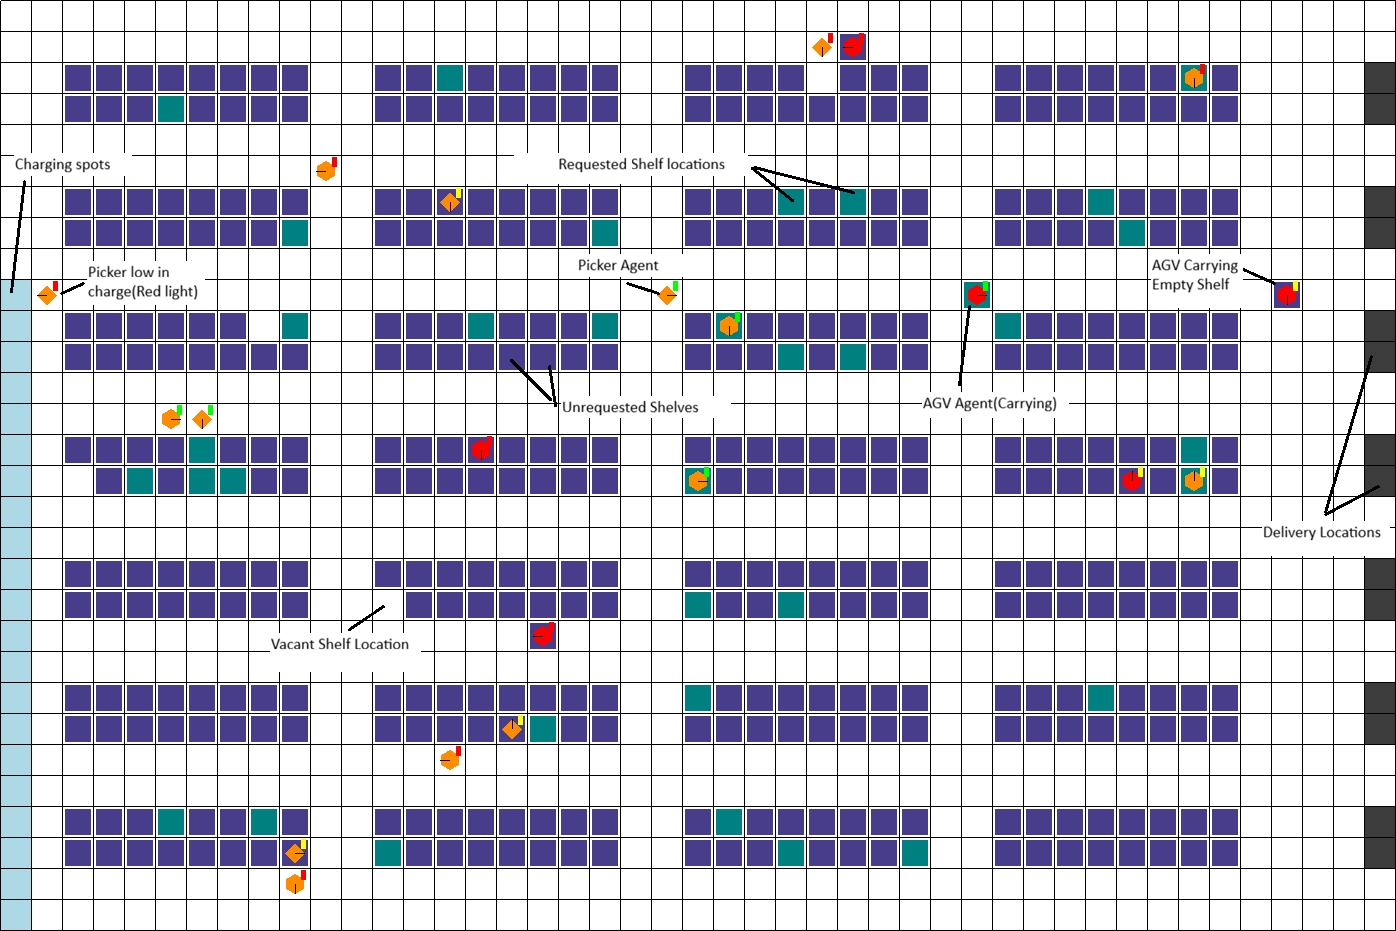
\includegraphics[width=0.95\textwidth]{../Battery-TA-RWARE/docs/img/BatteryTA-RWARE.png}
    \caption{Illustration of the task-assignment warehouse setting used in this thesis.}
    \label{fig:tarware_overview}
\end{figure}

The environment exposes a discrete action space where each action corresponds to selecting a target location:
\begin{itemize}
    \item \textbf{Shelf actions:} choose a shelf location (e.g., to pick up or return a shelf).
    \item \textbf{Goal actions:} choose a delivery station (primarily relevant when an \gls{agv} carries a requested shelf).
    \item \textbf{Charging actions:} choose a charging station to recover battery.
\end{itemize}
Low-level motion toward the selected target is handled internally by the environment (A* path planning and collision resolution), while the controller is evaluated on the quality of these high-level decisions.

\subsection{Language-Model Control Loop}
\label{sec:llm_loop}
The \gls{llm} policy is implemented as a text-in / discrete-action-out controller:
\begin{enumerate}
    \item \textbf{State summarization:} extract salient features of the global state (requested shelves and their action ids, per-agent position/target/battery/carrying status, charging occupancy).
    \item \textbf{Candidate action set:} compute a valid-action mask from the environment and derive the prompt-visible candidate set from those feasible actions. These candidates are presented as compact role-relevant action rows with action ids and guidance fields such as distance, tags, and charging-related instructions.
    \item \textbf{Prompting:} generate a per-agent prompt describing the agent role and the current state, including explicit mappings from requested objects to action ids.
    \item \textbf{Querying:} send the prompt to a local inference server (Ollama) and obtain a text response.
    \item \textbf{Parsing:} parse an integer action id (and optionally an action hold duration) from the response.
    \item \textbf{Validation:} validate the parsed action id against the current valid-action mask. If the proposed action is missing or invalid, the controller discards it and falls back to an idle action for that step; in the action-persistence setting, an invalid persisted action clears the hold and forces a new query.
    \item \textbf{Execution:} apply the validated joint action in the environment for one step (or hold the action for multiple steps, depending on configuration).
\end{enumerate}

\begin{figure}[H]
    \centering
    \begin{tikzpicture}[
        node distance=5mm,
        box/.style={draw, rounded corners, align=center, minimum width=0.7\textwidth, minimum height=8mm},
        arrow/.style={-Latex, thick}
    ]
        \node[box] (state) {State summary from the current environment step};
        \node[box, below=of state] (candidates) {Candidate shaping and feasible-action mask};
        \node[box, below=of candidates] (prompt) {Prompt construction for joint or per-agent planning};
        \node[box, below=of prompt] (query) {Language-model query};
        \node[box, below=of query] (parse) {Parse action identifier and optional hold duration};
        \node[box, below=of parse] (validate) {Validate against current constraints};
        \node[box, below=of validate] (execute) {Execute one environment step or continue a persisted action};
        \node[box, below=of execute] (feedback) {Observe step consequence and decide whether replanning is needed};
        \draw[arrow] (state) -- (candidates);
        \draw[arrow] (candidates) -- (prompt);
        \draw[arrow] (prompt) -- (query);
        \draw[arrow] (query) -- (parse);
        \draw[arrow] (parse) -- (validate);
        \draw[arrow] (validate) -- (execute);
        \draw[arrow] (execute) -- (feedback);
        \draw[arrow] (feedback.east) -- ++(2.2,0) |- (state.east);
    \end{tikzpicture}
    \caption{Schematic of the language-model control loop used in the experiments.}
    \label{fig:lm_control_loop}
\end{figure}

The controller is best described as a discrete-time, step-synchronous supervisory loop with conditional replanning.
The environment advances one simulation step at a time, and at each step the controller reevaluates agent state and action validity.
However, this does not imply that every agent is queried at every step.
Instead, the experiments use two related control schemes.

\begin{itemize}
    \item \textbf{Step-synchronous replanning with environment-owned continuation:} agents that are currently available for planning may receive a new high-level action, while busy agents are not replanned and continue their current task until the environment releases them.
    \item \textbf{Step-synchronous replanning with action persistence and conditional override:} accepted actions may remain active for multiple future steps, so agents are not re-queried while the persisted action remains valid. Replanning is triggered when a persisted action expires, becomes invalid, or when the controller decides intervention is needed, including selected busy-agent cases.
\end{itemize}

This design sits between two extremes.
A fully scheduled scheme that queries every agent at every step would generate many unnecessary \gls{llm} calls, while a purely event-triggered scheme is less natural in this setting because useful triggers such as blocked progress, invalid persisted actions, expiring commitments, or changing support needs are only known after the system state is checked.
The adopted design therefore combines regular per-step observability with selective replanning.
This is also consistent with practical supervisory control in warehouse systems, where the fleet is typically checked at regular intervals, ongoing tasks continue by default, and new task-level decisions are issued only when the current situation justifies intervention.

Two design choices are central for feasibility:
\begin{itemize}
    \item \textbf{Grounding via action ids:} the \gls{llm} does not output coordinates or free-form text commands; instead it selects from discrete action ids that are already defined by the environment.
    \item \textbf{Hard validation:} action masks enforce constraints such as invalid goals for picker agents and busy-state restrictions. Invalid \gls{llm} outputs are never executed.
\end{itemize}

The reported behaviour is therefore the behaviour of the complete control framework: prompt design, model output, candidate shaping, validation logic, and replanning policy act together inside the same supervisory loop.

\subsection{Experiment Design and Comparison Axes}
The experiments are organized as a controlled comparison within the grounded language-model control loop described above.
Across the experiment families, the environment, discrete action space, validation layer, scenario catalogue, local-inference setup, and evaluation metrics are kept as stable as practical.
The main factors that change are the objective formulation, model size, planning architecture, and prompt representation.
This structure is important because the thesis does not only ask whether an \gls{llm} can control the warehouse agents; it asks how different ways of using the \gls{llm} affect collaborative task performance under comparable conditions.

The objective families define the main progression of the experimental campaign.
The first family uses a delivery-only objective, where the controller is evaluated primarily on raw shelf-delivery throughput.
This establishes the baseline interpretation for the later experiments: the controller is expected to select high-level actions that move requested shelves through the warehouse as effectively as possible.
The second family keeps the same warehouse task and comparison axes, but changes the objective into a call-aware formulation that seeks to maintain delivery performance while reducing unnecessary \gls{llm} queries.
In this family, the output interface includes a \nolinkurl{Steps} field, allowing a selected action to persist for multiple simulation steps when repeated replanning is not useful.
The third family extends the same framework toward battery-aware control, where the purpose is to study whether the controller can incorporate resource constraints in addition to throughput and call efficiency.
Together, these objective families make it possible to compare not only absolute delivery performance, but also how the same supervisory loop behaves when the definition of a good decision changes.

Two planning architectures are compared inside this framework.
In the centralized architecture, one \gls{llm} call plans for all agents that currently need a decision, using a prompt that exposes the global state and the relevant candidate actions.
This gives the model an explicit opportunity to coordinate joint behaviour, but it also increases the prompt size and output complexity as the number of agents and candidate actions grows.
In the shared-context per-agent architecture, the model plans for one agent at a time.
Each prompt still contains global information, but the required output concerns only the current agent.
This reduces parsing burden and makes the decision format simpler, while shifting coordination from one explicit joint plan to a sequence of local decisions made with shared context.
The comparison is therefore meaningful because it separates two practical ways of embedding language models in multi-agent control: broad joint reasoning versus simpler repeated decisions.

Prompt representation is treated as another comparison axis rather than as a separate experiment in isolation.
The prompts always ground the model's choice in explicit action ids and role-relevant state, including requested-shelf mappings, rules for \glspl{agv} and pickers, support relations such as waiting-for-picker context, battery-state abstractions, and filtered or prioritized candidate actions.
What varies is the form in which the model is asked to respond, especially natural-language action selection versus structured \gls{json} output.
This comparison tests whether stronger output structure improves reliability without changing the underlying warehouse task.
Taken together, the principal comparison axes are model size, centralized versus shared-context per-agent planning, natural-language versus \gls{json} prompting, and the three objective formulations of delivery-only, call-aware delivery, and battery-aware control.

\subsection{Scenarios, Models, and Metrics}
The same scenario catalogue is reused across the experiment families so that differences in observed behaviour can be interpreted against known coordination pressures rather than against unrelated task changes.
The scenarios are \nolinkurl{tiny_balanced_1v1}, \nolinkurl{small_balanced_2v2}, \nolinkurl{medium_balanced_4v4}, \nolinkurl{small_agv_heavy_4v2}, \nolinkurl{medium_agv_heavy_6v2}, and \nolinkurl{small_picker_heavy_2v4}.
These scenarios cover simple balanced collaboration, increased concurrency, larger warehouse layouts, \gls{agv}-heavy settings where picker support can become a bottleneck, and picker-heavy settings where allocation efficiency and underutilization become more visible.
The scenario set therefore tests whether a model, prompt form, or planning architecture remains productive when the source of coordination difficulty changes.

The model set spans smaller and larger local models: \nolinkurl{llama3.2:1b}, \nolinkurl{llama3.2:3b}, \nolinkurl{mistral:7b}, \nolinkurl{gemma3:12b}, \nolinkurl{phi4}, and \nolinkurl{qwen2.5:14b}.
Using models of different sizes supports the thesis question about whether larger models produce better coordination, or whether smaller models can remain competitive when the prompt is sufficiently grounded and the validation layer prevents infeasible actions from being executed.
Because all models operate through the same discrete-action interface, the comparison concerns decision quality within the same controller framework rather than differences in low-level robot control.

The primary metric is delivery throughput, expressed as pick rate, which is computed from the number of delivered shelves and the simulated episode duration.
Total shelf deliveries are also reported directly because they are easy to interpret in relation to the task objective and the episode-level delivery ceiling.
Additional metrics are collected to explain how a controller reaches its throughput outcome: clashes, deadlocks or stuck events, distance travelled by each agent type, episode return, episode length, and inference speed or latency when measured.
These supporting metrics are necessary because two configurations can achieve similar delivery counts for different reasons.
For example, one configuration may maintain throughput with fewer model calls, while another may show the same delivery count but with more clashes, longer no-delivery tails, or inefficient movement.
The metrics therefore connect the numerical result to the underlying collaborative behaviour.

\subsection{Experimental Protocol}
The reported experiment sessions were run with fixed environment ids and a fixed seed, creating a controlled set of comparable runs for the reported objective families.
Within that controlled setup, the campaign proceeds from Objective~1 delivery-only experiments to Objective~2 call-aware delivery experiments and then to Objective~3 battery-aware experiments.
This ordering is deliberate.
The delivery-only experiments first establish how the models, prompt forms, and planning architectures behave when the objective is simply to complete warehouse deliveries.
The call-aware experiments then ask whether the same framework can reduce unnecessary replanning without losing the productive behaviour established in the first family.
The battery-aware experiments extend the evaluation to resource-sensitive decision making, where the controller must consider battery constraints as part of the same high-level assignment problem.

Section~\ref{sec:result_discussion} reports Objective~1 for the shelf-delivery comparisons, Objective~2 for the call-aware comparisons, and Objective~3 for the battery-aware objective.
In the current simulation setup, a run can achieve at most 20 deliveries, and the results chapter uses that ceiling to contextualize reported scores.

\subsection{Delimitations}
To keep the study focused and interpretable, the following delimitations apply:
\begin{itemize}
    \item The work is evaluated in a simulated warehouse environment rather than on physical robots.
    \item The controller is responsible only for high-level target selection; low-level navigation and collision handling are performed by the environment.
    \item The evaluated language models are prompted general-purpose models accessed through a local inference server and are not fine-tuned for this task.
    \item The reported experiments use fixed seeds and a limited number of completed sessions.
    \item Completed aggregate results are not yet available for the battery-aware objective family.
\end{itemize}

\subsection{Ethical and Sustainability Considerations}
Although the present work is simulation-based, it raises practical issues that remain relevant for real multi-robot deployments.
The primary ethical concern is safety and reliability: generated decisions may be infeasible, unstable, or unproductive if they are not constrained by system-side checks.
For that reason, the studied control loop does not execute free-form outputs directly. It uses grounded action identifiers, candidate shaping, explicit feasibility validation, and fallback behavior so that unsafe or clearly invalid actions are filtered before execution.
The logging of prompts, parsed outputs, executed actions, and observed step consequences also improves traceability, which is important when analyzing failures such as long no-delivery tails, stale waiting loops, or battery-related breakdowns.

From a sustainability perspective, the main trade-off is between model capability and computational cost.
Larger language models generally require more inference time and compute, while smaller models may require stronger prompt structure and validation to remain effective.
This thesis therefore treats call efficiency, unnecessary replanning, and coordination overhead as practically relevant concerns rather than only implementation details.
Even with safeguards, fixed-seed evaluation, limited scenario coverage, and the absence of physical deployment still bound the scope of the reported results.
